% small.tex
\documentclass[12pt]{beamer}
\usetheme{amcg}
\beamertemplatenavigationsymbolsempty
\renewcommand{\thefootnote}{}
\providecommand{\e}[1]{\ensuremath{\times 10^{#1}}}
\usepackage{mathptmx}
\usepackage{helvet}
\usefonttheme{serif}
\newcommand\TILDE{\char`\~}
\usepackage{listings}
\lstset{
        basicstyle              = \scriptsize\ttfamily,
        breaklines              = true,
        breakindent             = 10pt,
        breakatwhitespace       = true,
        breakautoindent         = true,
        keywordstyle            = \color[RGB]{0,0,255},
        commentstyle            = \itshape\color[RGB]{120,120,120},
        stringstyle             = \color[rgb]{0.627,0.126,0.941},
        emphstyle               = {[0]\color[RGB]{236,0,168}},
        emphstyle               = {[1]\color[RGB]{34,139,34}\underbar},
        emphstyle               = {[2]\textbf}
}
% items enclosed in square brackets are optional; explanation below
\begin{document}
 
\begin{frame}{Fluidity Training}
  \begin{center}
  {\Large Running Fluidity and Visualising the Results}
  \vspace{1.5cm}\\
  \large Simon Mouradian\\
  \vspace{0.2cm}
  11-13 November 2015
  \end{center}
\end{frame}

%-- Overview slide --- %
\section*{Outline}
\begin{frame}
  \frametitle{Outline}
  \tableofcontents
\end{frame}

\section{Running}
\begin{frame}
    \frametitle{Running Fluidity}

\texttt{\$ <trunk>/bin/fluidity my.flml}\\
\vspace{1ex}
If fluidity is installed on the system:\\
\texttt{\$ fluidity my.flml}

\vspace{1ex}
Common options:\\
-l \qquad (Create log file for each process)\\
-v N \qquad (Verbosity level, default level 0, N can be 0,1 or 2)\\
-h \qquad (Help)
\vspace{1ex}

Example:\\
\texttt{\$ fluidity -l -v2 my.flml}

\end{frame}

%% \begin{frame}[fragile]
%%     \frametitle{{\tt fluidity --help}}
%% \lstset{language=bash,basicstyle=\tiny}
%% \begin{lstlisting}[language=bash]

%% Revision: fluidity/4.1
%% Compile date: Nov 20 2012 10:16:12
%% OpenMP Support			no
%% Adaptivity support		yes
%% ...
%% FEMDEM support			no
%% Hyperlight support		no


%% Usage: fluidity [options ...] [simulation-file]

%% Options:
%%  -h, --help
%% 	Help! Prints this message.
%%  -l, --log
%% 	Create log file for each process (useful for non-interactive testing).
%%  -v <level>, --verbose
%% 	Verbose output to stdout, default level 0
%%  -p, --profile
%% 	Print profiling data at end of run
%% 	This provides aggregated elapsed time for coarse-level computation
%% 	(Turned on automatically if verbosity is at level 2 or above)
%%  -V, --version
%% 	Version
%% \end{lstlisting}
%% \end{frame}


\section{Output}

\subsection{Filetypes and tools}
\begin{frame}
    \frametitle{Output Filetypes}
Today we will look at two types:
\begin{itemize}
    \item Stat file (.stat)
    \item Unstructured VTK file (.vtu or .pvtu)
\end{itemize}
\vspace{5mm}
Fluidity also has a third filetype:
\begin{itemize}
\item Detectors (.detectors)
\end{itemize}
\vspace{5mm}
You may also have log files:
\begin{itemize}
    \item fluidity.log-*
    \item fluidity.err-*
\end{itemize}

\end{frame}

\begin{frame}
    \frametitle{Tools}
\begin{itemize}
\item Statplot
\item Paraview
\item Python
    \begin{itemize}
    \item fluidity.statparser
    \item vtktools
    \end{itemize}
\end{itemize}
\end{frame}

\begin{frame}
    \frametitle{Copy ``Top Hat'' example}

We're going to copy and run a ready--made example:

\vspace{5mm}
First, to prepare the files...\\
{\tt cp -rv /scratch/examples/top\_hat .}\\
{\tt cd top\_hat}\\
{\tt make clean}\\
{\tt make preprocess}

\end{frame}

\begin{frame}
    \frametitle{Run ``Top Hat'' example}

Type ``{\tt ls}'' to see the {\tt .flml} and mesh {\tt line.msh} files.
There are three separate set-up files and one mesh.

\vspace{5mm}
{\tt \$ fluidity -l -v2 top\_hat\_cg.flml \&}\\
\vspace{5mm}

After running Fluidity, the {\tt .vtu} files contain the results. Each {\tt .vtu} contains the output at a single time--level.

\end{frame}

\subsection{The stat file}

\begin{frame}
    \frametitle{The stat file}
\begin{columns}
\begin{column}{0.6\textwidth}
\begin{itemize}
\item Bespoke data file type
\item Various tools to read and process these data
\item Either ASCII or binary
\end{itemize}
\end{column}
\begin{column}{0.4\textwidth}
\begin{center}
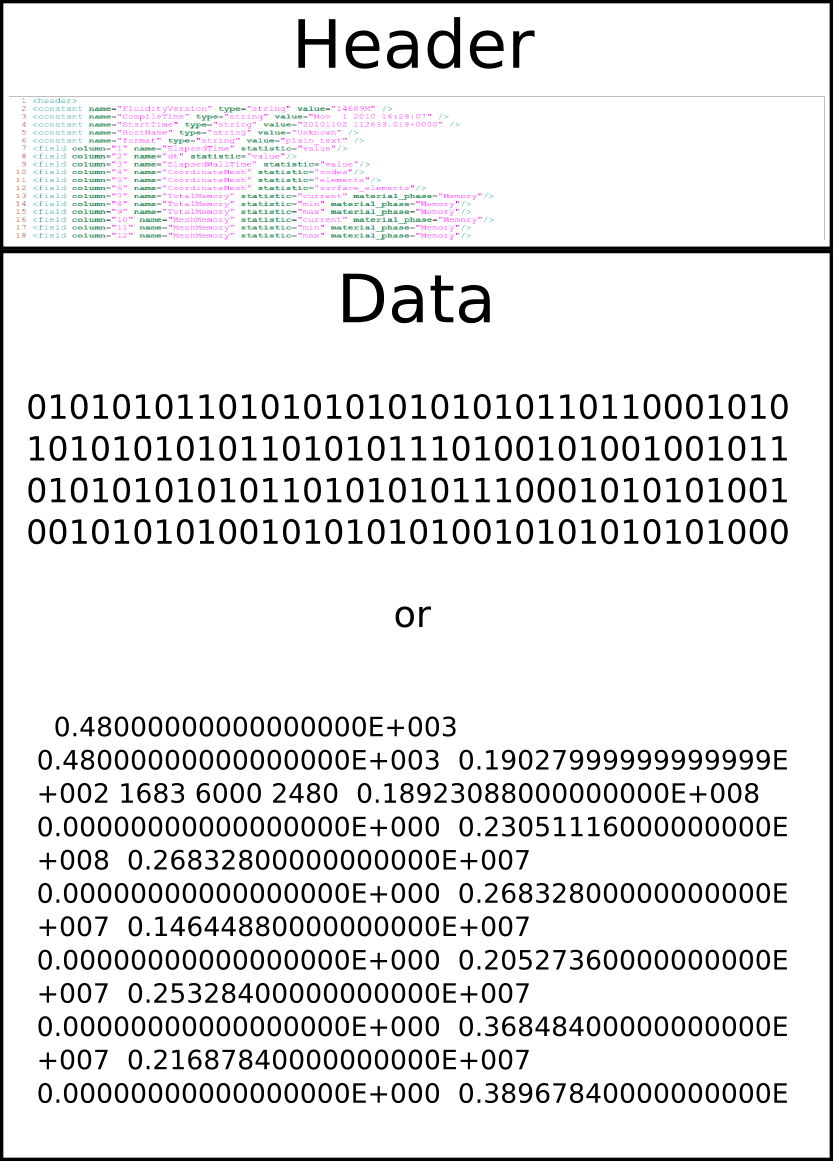
\includegraphics[width=0.7\textwidth]{images/stat_file.png}
\end{center}
\end{column}
\end{columns}
\end{frame}

\begin{frame}
    \frametitle{Statplot}
\begin{center}
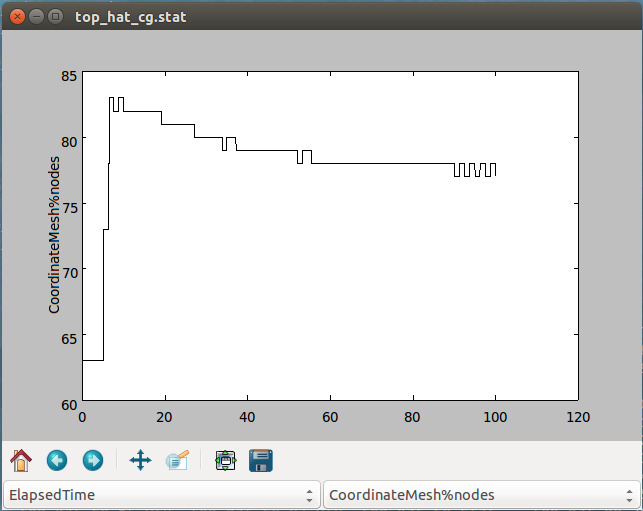
\includegraphics[width=0.6\textwidth]{images/statplot.png}\\
\end{center}
\texttt{\$ statplot top\_hat\_cg.stat}
\end{frame}

\begin{frame}
    \frametitle{Statplot}
\begin{center}
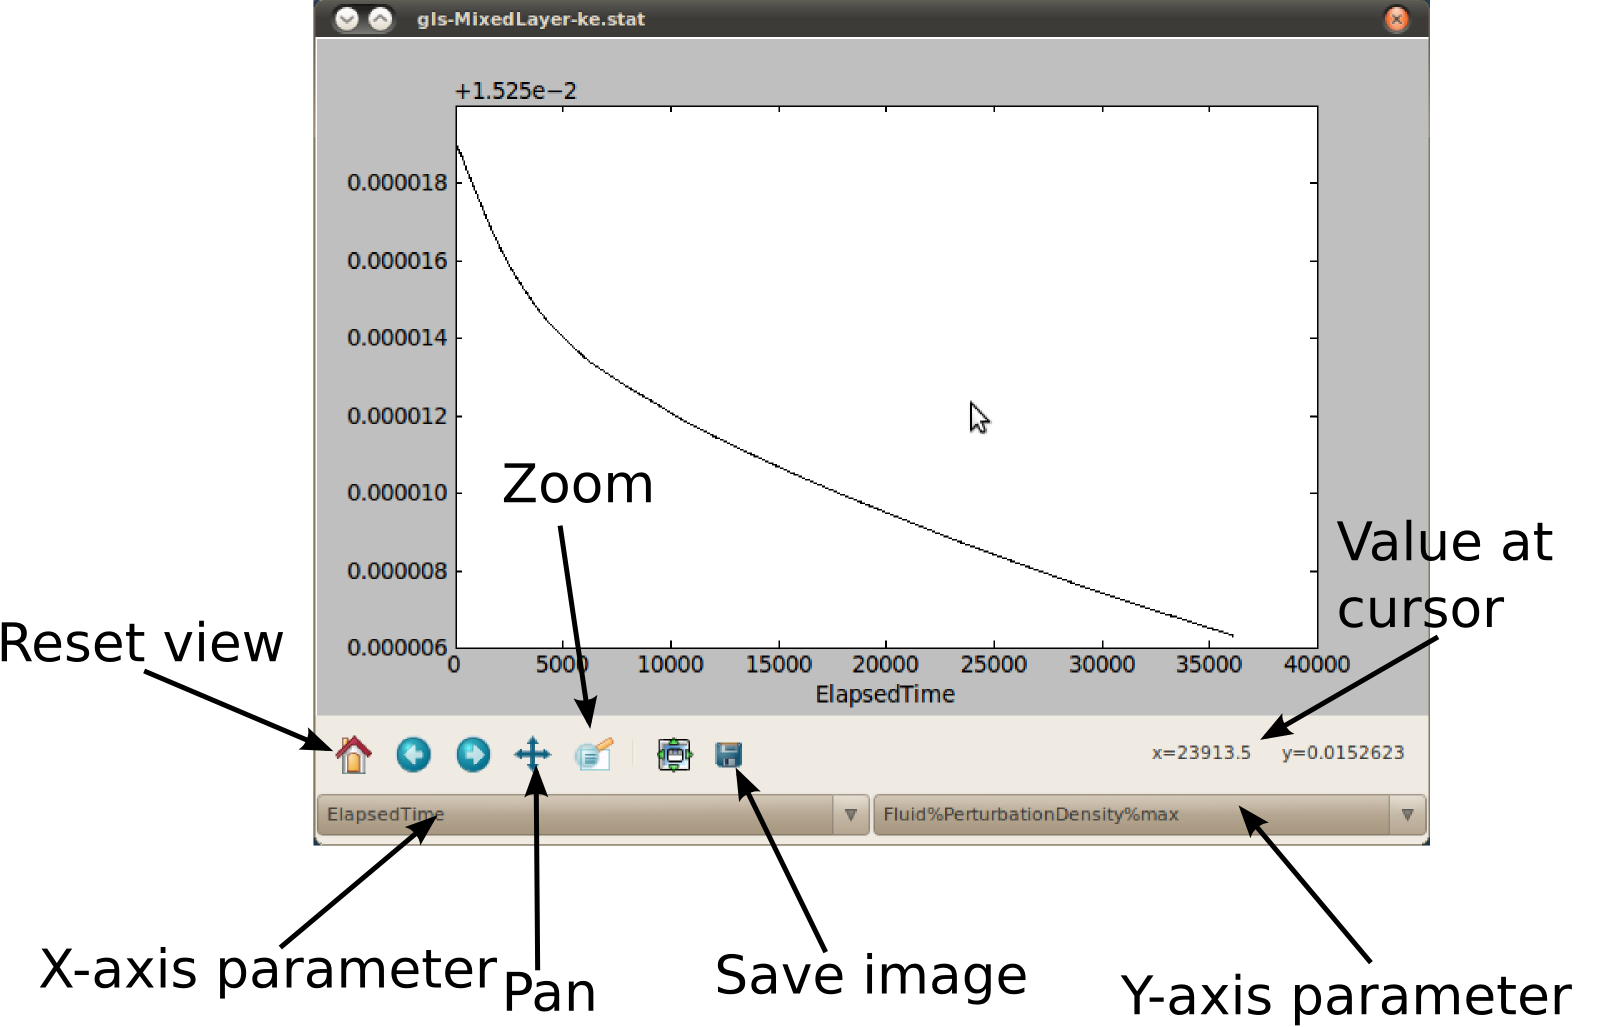
\includegraphics[width=0.8\textwidth]{images/statplot_labelled.png}
\end{center}
\end{frame}

\begin{frame}
    \frametitle{Statplot keys}
\begin{itemize}
\item s - scatter plot
\item l - line plot
\item r - refresh data
\item R - refresh data, but keep current bounds
\item x - switch x-axis from linear to log or vice versa
\item y - switch y-axis from linear to log or vice versa
\item q - quit (note: \textbf{no warnings!})
\end{itemize}
\end{frame}

\begin{frame}
    \frametitle{Statplot example}
Open the stat file at from your advection problem

Things to try:
\begin{itemize}
\item Switch between scatter plot and line plot views
\item Change the graph to show the number of elements through the run
\item Plot tracer maximum against time
\item Zoom in and save a small part of the plot to file
\end{itemize}
\end{frame}

\subsection{Paraview}
\begin{frame}
    \frametitle{Paraview}
Open--source scientific visualisation software from KitView
\begin{center}
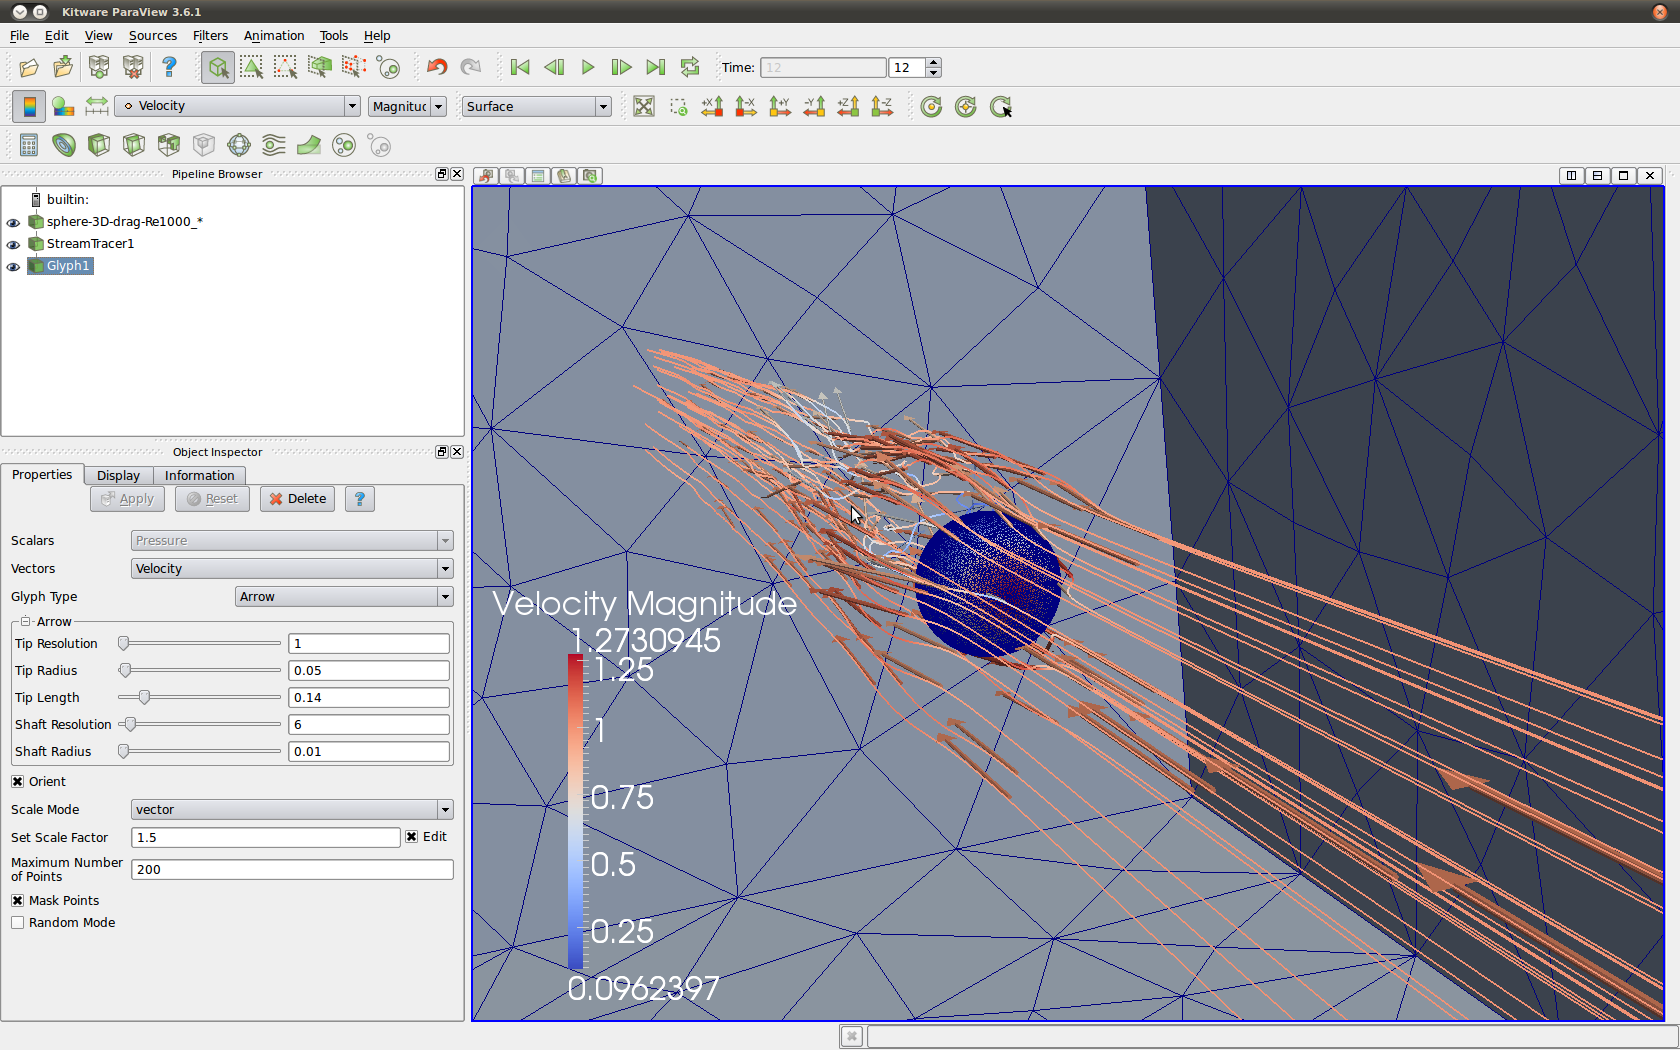
\includegraphics[width=0.6\textwidth]{images/paraview_example.png}\\
\vspace{5mm}
This can be obtained on your own machine using:\\
{\tt \$ sudo apt-get install paraview} $\leftarrow$ \emph{\color{red}But not now!}
\end{center}
\end{frame}

\begin{frame}
    \frametitle{Paraview: main window}
\begin{center}
Launch by simply typing ``{\tt paraview \&}''\\
\vspace{5mm}
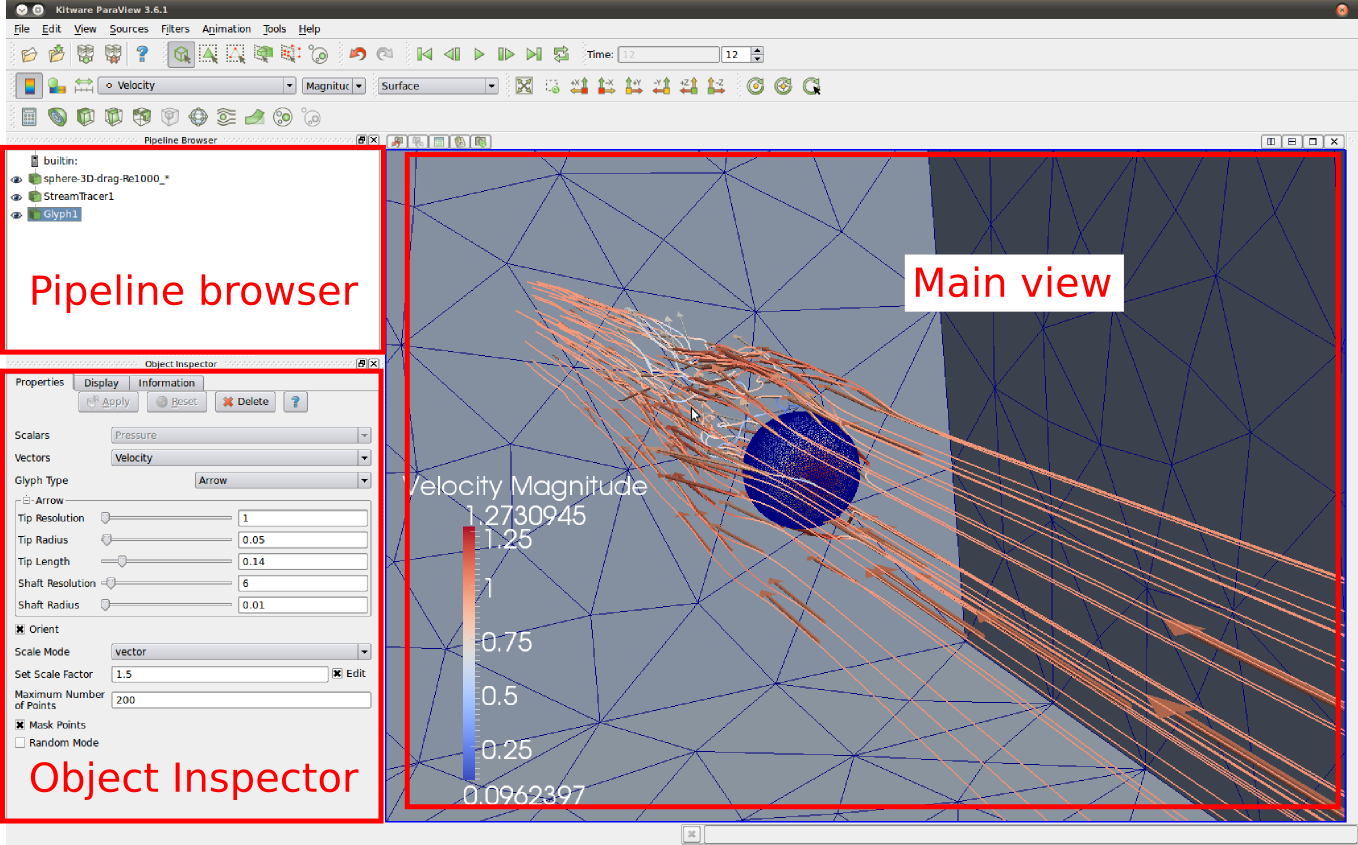
\includegraphics[width=0.7\textwidth]{images/paraview_window.png}
\end{center}
\end{frame}
\begin{frame}
    \frametitle{Paraview: main window}
\begin{center}
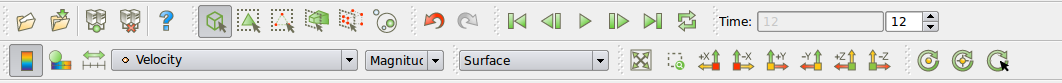
\includegraphics[width=\textwidth]{images/paraview_toolbar.png}
\end{center}
\end{frame}
\begin{frame}
    \frametitle{Paraview: Copy data for visualisation}
So we're going to copy across some ready-made data again
to play around with.\\
\vspace{5mm}
{\tt cd ..} \\
{\tt ls} \\
{\tt cp -rv /scratch/examples/backward\_facing\_step\_2d .}\\
{\tt cd backward\_facing\_step\_2d}\\
{\tt ls}

\end{frame}
\begin{frame}
    \frametitle{Paraview: Open files}
\begin{center}
\begin{itemize}
\item Click on ``OPEN'' icon
\item Navigate into ``backward\_facing\_step\_2d'' and then ``kepsilon''
\item Scroll to the bottom
\item Double-click on ``...pvtu'' file
\end{itemize}
\end{center}
\end{frame}

\begin{frame}
    \frametitle{Paraview}
\begin{center}
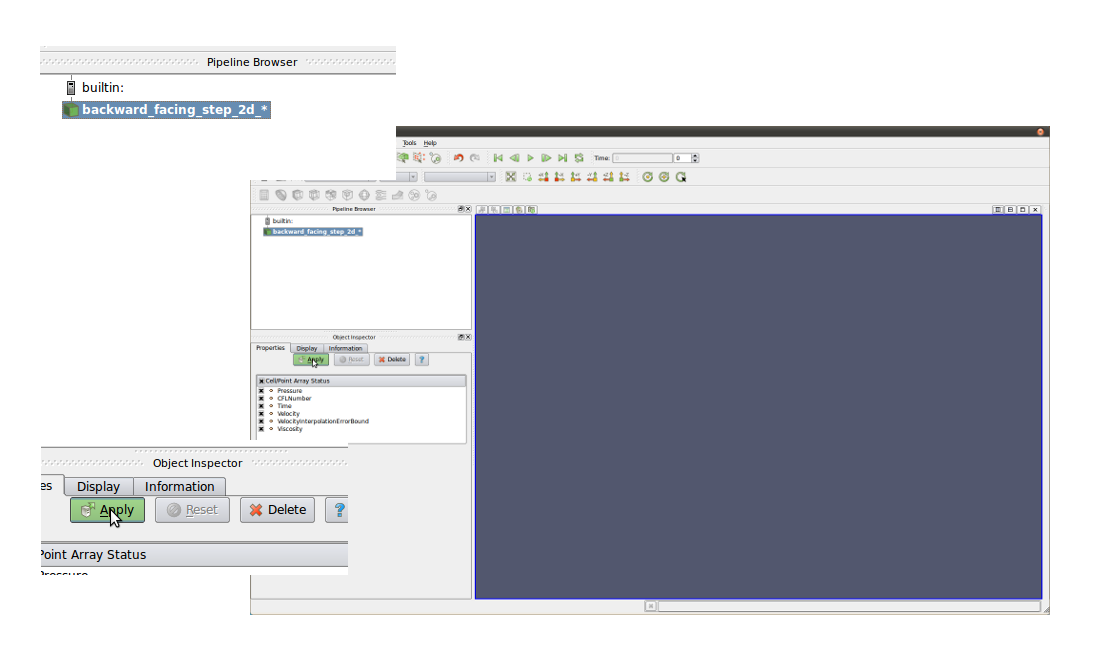
\includegraphics[width=\textwidth]{images/paraview_after_open.png}
\end{center}
\end{frame}
\begin{frame}
    \frametitle{Paraview}
\begin{center}
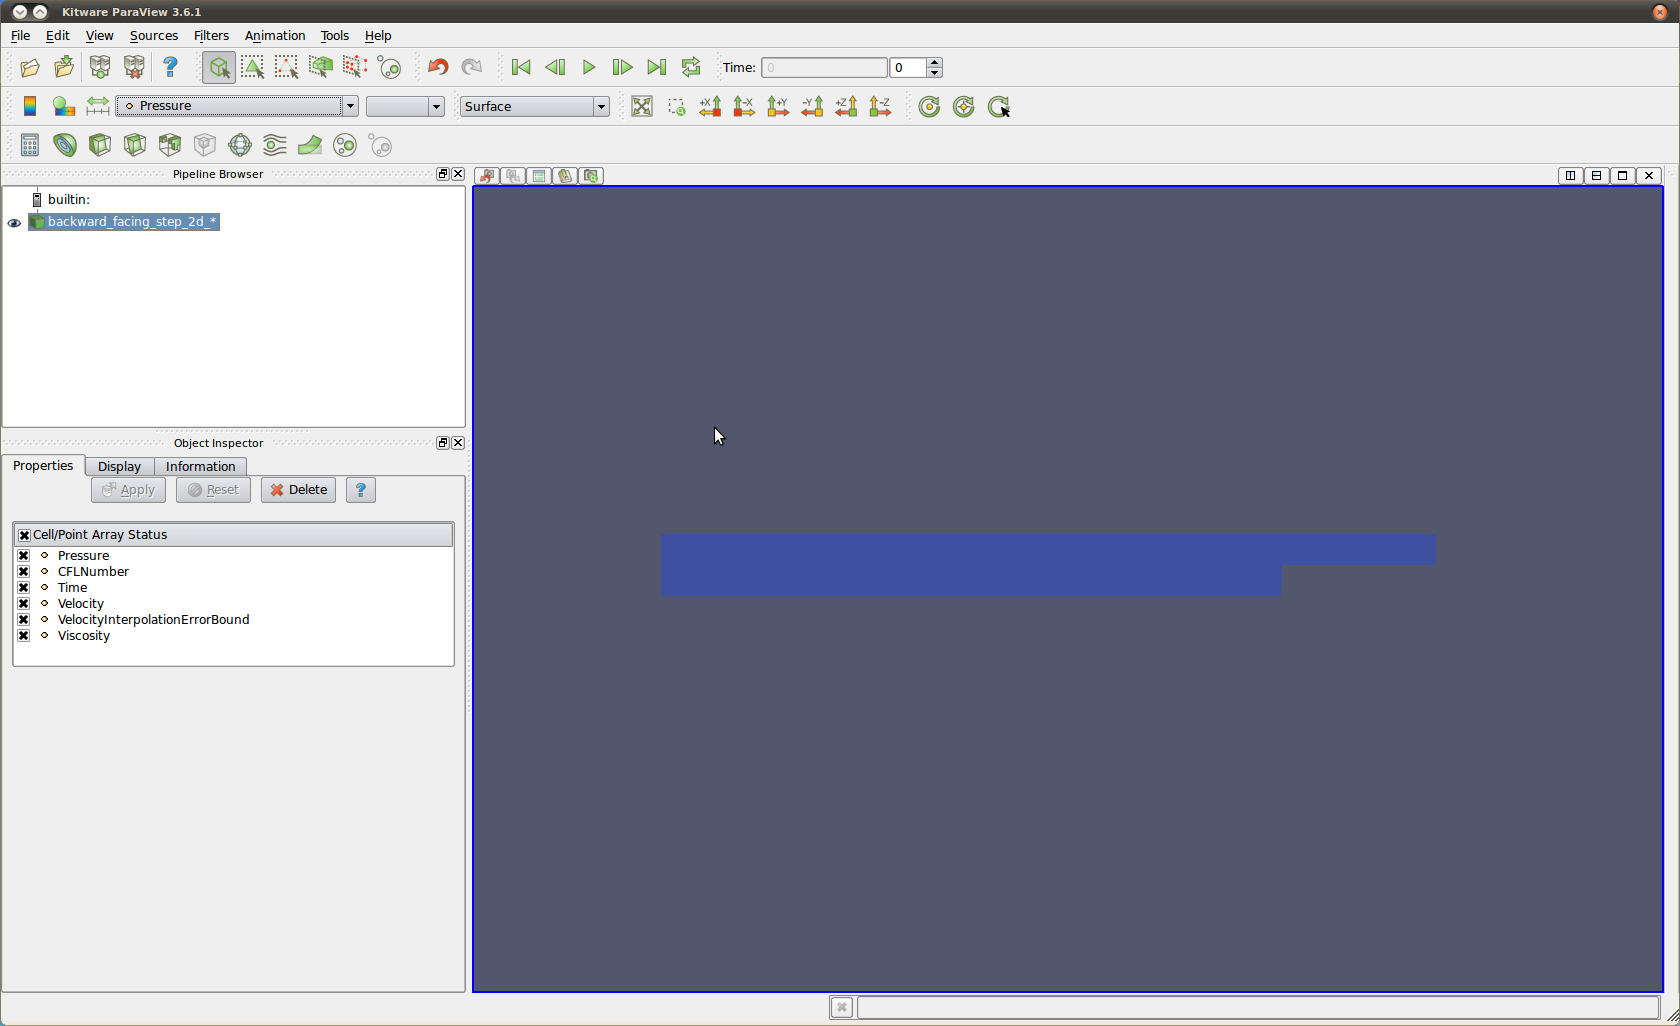
\includegraphics[width=0.75\textwidth]{images/paraview_after_loading.png}
\end{center}
\end{frame}
\begin{frame}
    \frametitle{Paraview}
\begin{itemize}
\item Right click: Zoom-in and out
\item Left-click: rotate
\item Middle-button: move
\item Use the drop-down menu to change field
\item Use the green arrow keys to change the timestep
\end{itemize}
You are likely to use Paraview a lot for visualisation of data
and learning to use it well is useful. Feel free to consult the Paraview
tutorials for further practice and worked examples:\\
\begin{center}
 {\tt www.paraview.org/Wiki/The\_ParaView\_Tutorial}
\end{center}

\end{frame}

\subsection{Python}
\begin{frame}
    \frametitle{Python tools}
\begin{itemize}
\item vtktools - read vtu files 
\item statparser - read stat files
\end{itemize}
\end{frame}

\begin{frame}
  \frametitle{Reading .stat file in Python}
\texttt{import fluidity\_tools} \\
\texttt{stat = fluidity\_tools.stat\_parser(filename)} \\
\vspace{5mm}
The stat object is a hierarchy of dictionaries! \\
\vspace{5mm}
\texttt{stat["Fluid"].keys()} \\
\vspace{5mm}
More info in the Fluidity manual section $9.4.2$
\end{frame}

\begin{frame}
  \frametitle{Reading .vtu files in Python}

\texttt{import vtktools} \\
\texttt{data = vtktools.vtu(’example.vtu’)} \\
\texttt{p = data.GetScalarField(’Pressure’)} \\

\vspace{5mm}
$p$ is now an array of the scalar field 'Pressure' \\
\vspace{5mm}
More info in the Fluidity manual section $9.3.1$
\end{frame}

\begin{frame}
    \frametitle{Post-processing Python script}
We have a ready--made post--processing script.\\
\vspace{5mm}
To view the script, type ``{\tt gedit postprocessor\_2d.py \&}''\\
\vspace{5mm}
If you don't know Python very well, don't worry, it's a very popular and easy language to pick-up.\\
\vspace{5mm}
To run the script, type:\\
{\tt make postprocess TYPE=reference}
\end{frame}

\end{document}
